Network topology defines how routers and processing elements are connected in a network, and it directly affects communication performance, hardware cost, and scalability. Common network topologies include shared-bus, crossbar, ring, fat-tree, torus, and mesh, as shown in Figure~\ref{fig:network_topology} \cite{becker2012efficient}. Among them, shared-bus and ring have relatively simple structures but limited scalability, while crossbar provides high connectivity at the cost of large hardware overhead. Mesh and torus are more suitable for scalable systems because of their regular structure and simple routing. In particular, mesh topology is widely used due to its good balance between performance, implementation complexity, and layout regularity. Therefore, a $3 \times 3$ two-dimensional mesh topology is adopted in this thesis as the target network structure for communication among processing elements.

\begin{figure}[htbp]
    \centering
    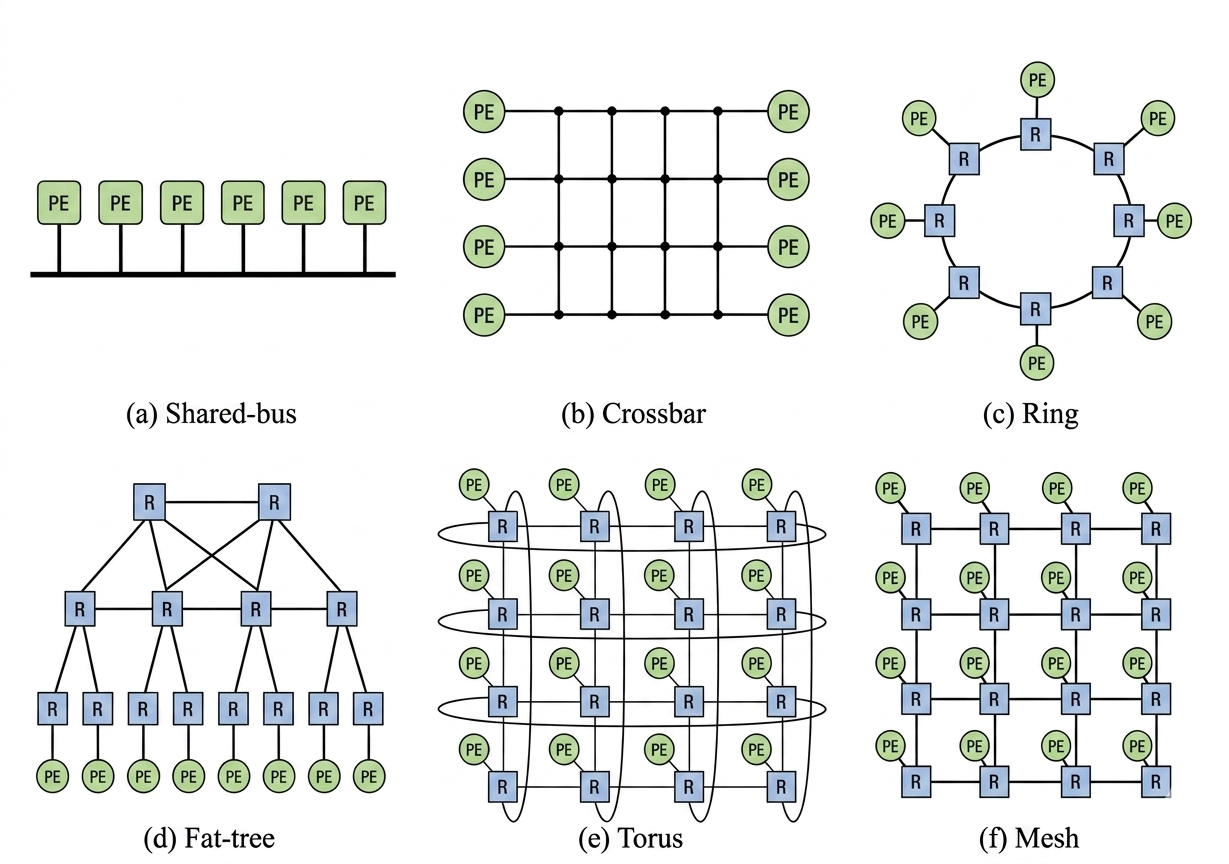
\includegraphics[width=0.8\textwidth]{images/ch2background/network_topology.png}
    \caption{Network topology}
    \label{fig:network_topology}
\end{figure}
